\RequirePackage[l2tabu, orthodox]{nag}
\documentclass[a4paper, twocolumn]{article}
\usepackage[english]{isodate}
\usepackage[utf8]{inputenc}
\usepackage[T1]{fontenc}
\usepackage{lmodern}
\usepackage[pdftex, hidelinks,
            pdftitle={Behaviour Tree Evolution by Genetic Programming},
            pdfauthor={Martin Estgren and Erik S. V. Jansson},
            pdfsubject={Artificial Intelligence - Genetic Programming},
            pdfkeywords={artificial intelligence, genetic programming,
                         behaviour trees, a-star, shooter}]{hyperref}

\usepackage{bm}
\usepackage{caption}
\usepackage{listings}
\usepackage{booktabs}
\usepackage{mathtools}
\usepackage{algorithmic}
\usepackage{multicol}
\usepackage{graphicx}
\usepackage{courier}
\usepackage{amsmath}
\usepackage{amssymb}
\usepackage{algorithm}
\usepackage[capitalize, noabbrev]{cleveref}
\usepackage[activate={true, nocompatibility}, final,
            tracking=true, kerning=true, spacing=true,
            factor=1100, stretch=10, shrink=10]{microtype}

\newcommand\blfootnote[1]{%
    \begingroup
        \renewcommand\thefootnote{}\footnote{#1}%
        \addtocounter{footnote}{-1}%
    \endgroup
}

\DeclareCaptionFormat{modifiedlst}{\rule{\textwidth}{0.85pt}\\[-2.9pt]#1#2#3}
\captionsetup[lstlisting]{format =  modifiedlst,
labelfont=bf,singlelinecheck=off,labelsep=space}
\lstset{basicstyle=\footnotesize\ttfamily,
        breakatwhitespace = false,
        breaklines = true,
        keepspaces = true,
        language = Java,
        showspaces = false,
        showstringspaces = false,
        frame = tb,
        numbers = left,
        numbersep = 5pt,
        xleftmargin = 16pt,
        framexleftmargin = 16pt,
        belowskip = \bigskipamount,
        aboveskip = \bigskipamount,
        escapeinside={<@}{@>}}

\title{\textbf{Behaviour Tree Evolution by Genetic Programming}\\
       \Large{\emph{-- Learning Novel Bot Behaviours in a 2D Top-Down Arena Shooter --}}}
\date{Linköping University, \today}
\author{{\textbf{Martin Estgren}} \;\;\;\;\;\;\;\;\;\, {\href{mailto:mares480@student.liu.se}
                                                       {\texttt{<mares480@student.liu.se>}}} \\
        {\textbf{Erik S. V. Jansson}} \;\;\;\;         {\href{mailto:erija578@student.liu.se}
                                                       {\texttt{<erija578@student.liu.se>}}} \\~\\
        \vspace{-5.0ex}}

\begin{document}
    \maketitle
    \section*{Abstract}

    Behaviour trees are a popular model for representing the decision-making and plan execution process for NPCs in video games. These are built by hand, and often require expertise to craft into interesting and intelligent behaviours. These types of behaviour trees usually don't adapt well to new environments, and need many tailor-made trees for each situation.

    In this paper we demonstrate how to generate the trees by using genetic programming; allowing us to essentially evolve novel behaviours automatically in our testbed. Instead of specifying low-level actions and conditions, we use high-level definitions. This leads to faster fitness convergence, and also allows us to skip the bloat control and tree pruning steps used by other similar behaviour tree evolution methods. Results show that the evolved trees reliably defeats our hand-crafted behaviours by the \(20^{th}\) generation.

    \vspace{1em}

    \begingroup
    \def\addvspace#1{}
    \tableofcontents
    \endgroup

    \section{Introduction} \label{sec:introduction}

    In interactive media such as video games, there is often a need for simulating seemingly complex agent behaviours in (soft) real-time. In a modern fast-paced computer game for example, the render, physics and artificial intelligence updates all need to complete in a total of less than 16ms to provide a half-decent experience. These resource constraint have spawned some very clever techniques to enable complex behaviours for autonomous agents while minimizing their required computational time.

    These techniques often require the bot behaviours to be manually defined, and in some cases, are quite hard to extend when new behaviours are needed later in the game development process. This has been shown to be true by industry researchers, such as \emph{Dawe et al}~\cite{dawe2014overview}, regarding the \emph{finite state machine architecture} (which we talk more about later).

    In this project we have explored how one of the more widely used techniques, \emph{behaviour trees}, can be extended to allow for not only hand-crafted complex behaviors, but for organic behaviours, tailored to the specific game domain by using a \emph{reinforcement learning} approach. More specifically, we evolve the behaviour trees by using \emph{genetic programming}. It's by no means a novel approach, but there still has been relatively little research in the area. In our \emph{behaviour evolution algorithm}, based on the work of \emph{{\"O}gren et al.}~\cite{colledanchise2015learning}, we instead use \emph{high-level behaviours}, which removes the need for \emph{bloat control} or \emph{pruning}. Leading to a simpler algorithm than \emph{{\"O}gren et al.}~\cite{colledanchise2015learning}.

    Alongside the proposed method in \cref{sec:proposed_approach}, a testbed consisting of a top-down arena shooter was built. It features a sufficiently complex environment to support interesting behaviours by the enemy bot. We describe the features of our testbed in \cref{sec:results_and_screenshots}.

    This report starts off in \cref{sec:background_theory} by giving a brief overview of the relevant techniques and related work necessary to follow our reasoning and findings. In \cref{sec:implementation_details} we describe the details needed to implement these techniques in practice, along with the testbed architecture we've used. This gives the reader information on any peculiarities and pit-falls. We follow this by showing in \cref{sec:results_and_screenshots} the testbed, and give some generated offspring generated by our method along with measurements of its efficiency. Finally, we reflect on our method, giving downsides, and present some possible future work in \cref{sec:discussion_and_outlook}.

    \subsection{Proposed Approach} \label{sec:proposed_approach}

    Apply \emph{genetic programming} to the \emph{behaviours trees} by creating \emph{high-level actions and conditions} nodes. Ideally this should allow for faster convergence rates and somewhat shallower generated behaviour trees, eliminating the need for \emph{bloat control} and \emph{pruning}. Since BTs are trees, the \emph{mutation mechanism} should modify \emph{control-flow structure} and \emph{leaf-node settings}, while the \emph{crossover mechanism} will swap sub-trees.

    \section{Background Theory} \label{sec:background_theory}

    For an autonomous agent to give the illusion of being intelligent, many different systems need to interact with each other. In this chapter we describe the theory behind our three primarily used techniques: \emph{behaviour trees}, \emph{path finding}, \emph{genetic programming}. There are entire books written on these techniques, hence we'll only describe each of these superficially, if you want a deeper treatment, see our references.

        \subsection{Behaviour Trees} \label{sec:behaviour_trees}

        Defining an accurate \emph{automatic planner} model is often impractical and usually overkill for real-world applications. Especially in games, where very simple models are enough to give the illusion of intelligence. In games, the most well-known \emph{behaviour selection algorithms} are \emph{FSMs}, \emph{GOAPs}, \emph{HTNs} and \emph{BTs} \cite{dawe2014overview}.

        \emph{Finite State Machines (FSMs)} are simple but hard to extend with additional states, resulting in an exponential increase of transitions \cite{dawe2014overview}. While both \emph{GOAP (Goal-Oriented Action Planner)} and \emph{HTN (Hierarchical Task Network)} are powerful models, these don't allow agents to explore new task definitions, and ``only'' provide an agent with novel ways of solving an already defined set of task. Planning has seen some use in the games industry. Most notably in the game \textit{F.E.A.R}~\cite{orkin2006three} where adversarial agents used a planning system to combat the player.

        \emph{Behaviour Trees (BTs)} on the other hand, when comparing to FSMs, provide advantages in terms of modularity, reactiveness and scalability. And more importantly, since they are a type of tree, allow for integration with the genetic programming approach. They were first popularized in \emph{Halo 2} \cite{isla2005managing}, but are now applied in other area as well, such as robotics.

        \emph{Behaviour Tree Evolution (BTE)} is a technique which uses some form of genetic programming on BTs. It's a relatively new technique that has been applied to \emph{strategy games} and \emph{platformers}. Some of the previous work is due to \emph{Lim et al.}~\cite{lim2010evolving}, \emph{Colledanchise et al.}~\cite{colledanchise2015learning} and a recent thesis by \emph{Hoff et al.}~\cite{hoff2016evolving}. To our knowledge, our paper is the first to attempt to apply BTE in a \emph{shooter game}, and also the first to use \emph{high-level behaviours} for a simpler algorithm.

        In the \emph{Behaviour Tree Starter Kit}~\cite{champandard2014behaviour} and also in \emph{Chris Simpson's Gamasutra article}~\cite{simpson2014behavior}, the BT is a tree-like data structure which describes the decision-making process of the agent. It's evaluated pre-order from the root of the tree, in each logic update tick.

        \begin{figure}[H]
            \centering
            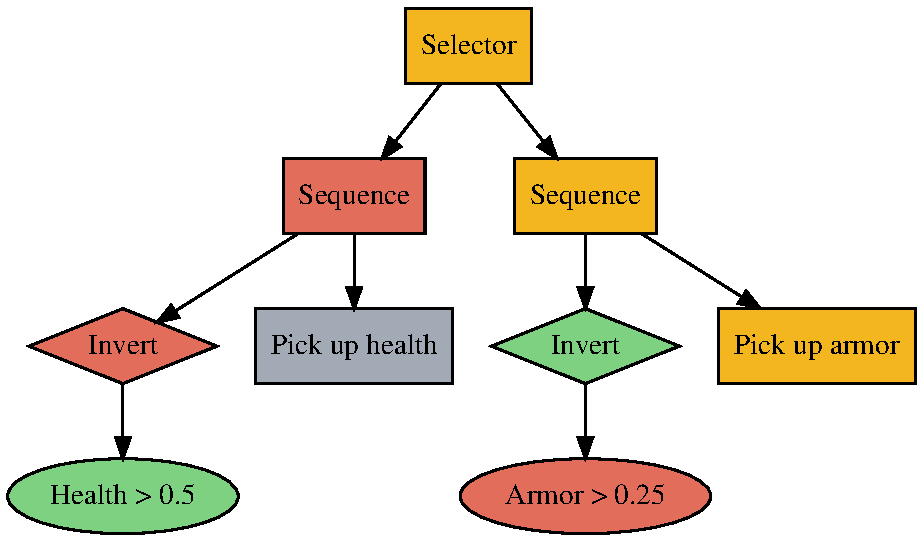
\includegraphics[width=\linewidth]{share/behaviour_tree.pdf}
            \caption{Example of Hand-Crafted Behaviour Tree}
            \label{fig:behaviour_tree}
        \end{figure}

        In the coming page you'll find the most common types of \emph{concrete nodes} in a behaviour tree, in particular those found in the \emph{BTSK}~\cite{champandard2014behaviour}. Only \emph{action} and \emph{condition nodes} are \emph{leaf-nodes}, and are \emph{concrete nodes}. All others are either \emph{composite or decorators} (\emph{abstract nodes}), which need to be instantiated to become concrete, such as the \emph{sequence} or \emph{inverter}; that have one/more children (it's never a leaf node).

        \begin{itemize}
            \item{\textbf{Selector:} executes children from left \(\rightarrow\) right until \emph{one child} is found to be either \emph{running} or has already \emph{succeeded}, and returns this status. Otherwise, if none matches, it returns a \emph{failure}.}
            \item{\textbf{Sequence:} executes children from left \(\rightarrow\) right until \emph{one child} is found to be either \emph{running} or \emph{failed}, and returns this status. If \emph{all children} have \emph{succeeded}, then also set status to \emph{success}.}
            \item{\textbf{Inverter:} executes the child node and \emph{inverts the resulting state} when it has finished running.}
            \item{\textbf{Succeeder:} when child has finished running, returns \emph{success} regardless of the child's status.}
            \item{\textbf{Condition:} a leaf-node that queries the world state, if the query returns true, we give \emph{success}, if it's false, we instead give \emph{failure}. This node is usually instantaneous, and can't be \emph{running}.}
            \item{\textbf{Action:} a leaf-node which modifies the world state, and returns \emph{success} if the action had the intended side-effect, \emph{failure} if couldn't complete or failed the action and \emph{running} if not done yet.}

        \end{itemize}

        We find that it's easier to understand behaviour trees with an example. We'll be using the tree in \cref{fig:behaviour_tree} as an example (it was produced within our testbed using a Graphviz library for Java). The yellow nodes means the node state is \emph{running}, the \emph{red} nodes have \emph{failed}, and \emph{green} nodes have \emph{succeeded}.

        At a high-level, this BT checks the agent's health and armour, and if it's below a threshold, it will go and pick up the crates which replenish these stats.

        It does this by starting at the root node, \emph{selector}, and executing the left child, the \emph{sequence}. It will also execute its left child, which is the \emph{inverter}. At last we reach a leaf-node, the \emph{health condition node}. This will probe the world for the state of the agent, and return \emph{success} because we've found that it's above 50\%. This result will propagate upward to its parent, the inverter, which will set its state to \emph{failed} (inverting the result of the child). We're back at the left sequence, and because one of the children have failed (the inverter), the sequence has \emph{failed} as well, and won't run the right child (gray means the node has never been evaluated). Finally, because the selector's left child has \emph{failed}, we execute the right branch too (remember, at least one child must succeed!). We use the same process before, but get stuck in \emph{``pick up armor''} until that action has finished \emph{running} in the world (has succeeded or failed).

        \subsection{Path Finding with A*} \label{sec:path_finding}

	Agent path finding is done using the \emph{A*} graph traversal algorithm proposed by Peter E. Hart, Nils J. Nilsson, and Bertram Raphael ~\cite{hart1968formal} as an extension to \emph{Dijkstra's algorithm} which, given an \emph{admissible heuristic} and non-negative costs, will find the path from a node \(n_0\) to a node \(n_g\), with the lowest cost.
	
    Calculating the expected cost of a path \(n_0 \rightarrow n_k \rightarrow n_g\), from \(n_0\) to \(n_g\) via \(n_k\) can be done with the following path finding cost function:
	\begin{equation*}
		f(n_k) = g(n_k) + h(n_k)
	\end{equation*}	
	where \(g(n_k)\) is the true cost from \(n_0\) to \(n_k\) and \(h(n_k)\) is a heuristic approximation of the cost from \(n_k\) to \(n_g\). This allows us to explore the potentially most optimal paths first before considering the others.

        In this project, the \emph{Euclidean distance} is used as the heuristic \(h(n_k)\). This, since the path finding is performed in a search-space where each node is defined as a point in the testbed's 2-D world-space.

    Additionally, compared to regular \emph{A*}, the path-finder also utilizes an \emph{influence map} to help the agent avoid ``suicidal paths'', even if the selected path is optimal given the heuristic function. Our \emph{influence map}, like the ones shown in \emph{Dave Mark}~\cite{mark2015modular}, take into account the visibility of each node in relation to the adversarial game agents' line-of-sight, and therefore updates the expected cost as:
	\begin{equation*}
		f(n_k) = g(n_k) + h(n_k) + i(n_k)
	\end{equation*} 
    where \(i(n_k)\) is the cost introduced by the influence map. This gives the the result that nodes within the adversarial agent's line-of-sight have a much higher associated traversal cost, and should be avoided. 
    \begin{minipage}{\linewidth}        	
    \centering
	\begin{minipage}{0.45\linewidth}
	\begin{figure}[H]
        \centering
		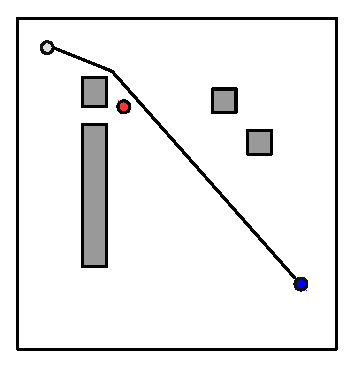
\includegraphics[width=\linewidth]{share/bad.eps}
		\caption{optimal path}
		\label{fig:optimal_path}
        \end{figure}
	\end{minipage}
	\hspace{0.00\linewidth}
	\begin{minipage}{0.45\linewidth}
	\begin{figure}[H]
        \centering
		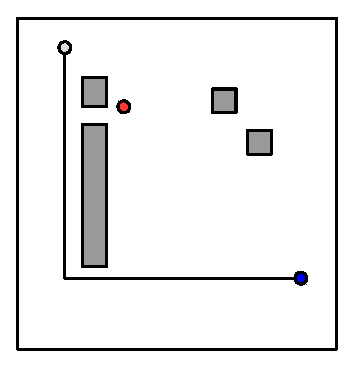
\includegraphics[width=\linewidth]{share/good.eps}
		\caption{tactical path}
		\label{fig:smart_path}
	\end{figure}
	\end{minipage}
\end{minipage}

\vspace{0.5em}

    Above are two example figures: \cref{fig:optimal_path} shows an optimal path using regular \emph{A*}, and the other, \cref{fig:smart_path} shows the optimal path when taking into account the influence map; sneaking behind cover.
	
	\subsection{Genetic Programming} \label{sec:genetic_programming}

    In many scenarios you try to optimize a function: \(f(x_0,x_1,...,x_n)\), where some or all of the inputs are of a discrete nature (ordinal or nominal values). These types of problems are often hard to optimize using techniques developed for continuous variables, such as \emph{gradient ascent/descent}, e.g. in a \emph{perceptron}.

	\emph{Genetic programming} is a technique that was introduced by \emph{Barricelli et al}~\cite{barricelli1954esempi}, as a way to optimize computer programs by encoding the parameters to be optimized as \emph{genetic representations} which could be processed by traditional \emph{evolutionary algorithms}.

	\begin{figure}[H]
        \centering
		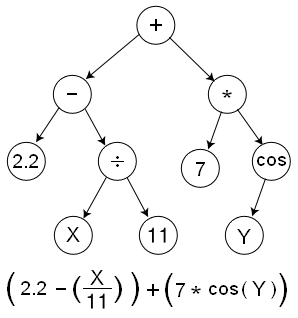
\includegraphics[width=0.5\linewidth]{share/Genetic_Program_Tree.png}
        \caption{The \emph{genetic representation} is often done using a tree-like structure in \emph{genetic programming}. Image is taken from: \texttt{\href{https://upload.wikimedia.org/wikipedia/commons/7/77/Genetic\_Program\_Tree.png}{Wikipedia}} (public domain).}
		\label{fig:genetic_representation}
	\end{figure}

	The most general form of the \emph{evolutionary algorithm} can be described in the following steps:
    \begin{enumerate}
        \item Generate an initial population by creating a initial pool \(\mathcal{P}_0\), of individuals with randomized genetic representations (context-specific data).
        \item Evaluate the \emph{fitness} for each individual \(x_i \in \mathcal{P}_t\). This usually requires a domain-specific \emph{fitness function}: \(f(x_i)\rightarrow f_i \in \mathbf{R}\), which will be described in further details later in this chapter.
        \item Remove individuals with poor \textit{low fitness score} and \emph{regenerate} population pool: \(\mathcal{P}_{t+1} = \Phi(\mathcal{P}_t)\).
    \end{enumerate}

    The fitness function for this project is composed of a \emph{linear combination} of desirable behaviours collected during the \emph{fitness evaluation} simulation, such as, amount of \emph{damage dealt} to the adversary, whether the agent with a specific BT \emph{survived}, and how many \emph{weapons the agent has picked-up}. In the implementation section we'll specify \(f_i\) more concretly, for now we just explain the general theory behind genetic programming and how to select \(\mathcal{P}_{t+1}\).

	\emph{Regeneration} of the population pool for the next generation, \(\mathcal{P}_{t+1}\), is done using the three functions:

    \vspace{1em}

    \textbf{Selection} ~ \(\Phi_s(\mathcal{P}_t) \rightarrow x_i \in \mathcal{P}_t\) ~ individuals with high \emph{fitness score} in the new population \(\mathcal{P}_{t+1}\). In this project, \emph{selection} is done proportionally to the \emph{fitness score} for each individual. Each individual \(x_i\) has a probability \(P(x_i|f_i)\) to be selected for the next generation \(\mathcal{P}_{t+1}\) according to some random process.
    \begin{equation*}
        P(x_i|f_i) = \frac{f_i}{\sum_{j = 1}^{N}f_j} \; \; \text{where} \; \; N = |\mathcal{P}_t|
    \end{equation*}

    \textbf{Crossover} ~ \(\Phi_c(x_i,x_j) \rightarrow \hat{x}_i,\hat{x}_j\) ~ individuals from the new population which have been crossed over, in the case of \emph{genetic programming}, \emph{crossover} is done by swapping random \emph{sub-trees} in each BT. All sub-trees has an equal probability of being selected to crossover, creating new individuals in \(\mathcal{P}_{t+1}\).

    \vspace{1em}

    \textbf{Mutation} ~ \(\Phi_m(x_i) \rightarrow \hat{x}_i\) ~ a subset of the new population, but slightly tweaked with a random parameter or by adding/removing random child nodes. If no mutation is done, then the genetic programming might converge to some local optima because of monoculture, and never reach a global optimum.

    \vspace{1em}

    Once these steps have been performed, a new generation of individuals have been produced, which can then be used to repeat the optimization process until we converge to a population with behaviours close the global maximum of the fitness function \(f_i\).


    \section{Implementation Details} \label{sec:implementation_details}

        After presenting these theoretical methods we'll now describe the additional changes necessary to make these work in practice (as per our implementation).

        Both the top-down shooter game (target \emph{testbed}) and our \emph{behaviour tree evolution} (the \emph{technique}) are written in \emph{Java} and use \emph{libGDX} for graphics/audio. This has allowed us to quickly produce a prototype, and while the game itself isn't the main topic of this paper, a rough outline can be found in \cref{sec:game_architecture}.

        Every \emph{entity} in the game can be transformed into an intelligent agent with a \texttt{BotInputComponent}, which associates a given \emph{behaviour tree} with a entity. It hooks together with the \emph{path finder} to enable the entity to \emph{traverse \& interact} with the environment. With GP, additional BTs can be generated and used.

        \subsection{Game Architecture} \label{sec:game_architecture}

        Given the very limited implementation time of this project, the architecture of the game was designed to allow for fast prototyping iterations, and isn't necessarily based on strong and scalable software design philosophies. The structural design is based on the \textit{entity component system} design, which has seen high use in the contemporary games industry and is being used in high-profile projects such as the \textit{Unity} game engine. The primary reference implementation is taken from the book \textit{Game Programming Patterns} written by \textit{R. Nystrom}~\cite{nystrom2014game} remixed with the component system from \textit{M. Boström}s' \textit{Speed Coding Zelda}~\footnote{\url{www://github.com/MilleBo/SpeedCodingZelda}}. The resulting implementation can be seen in the source code in the package: \texttt{se.sciion.quake2d.level} and its sub-folders.

        An \textit{entity component system (E-C-S)}, as the name might suggest, consists of three interacting class types. The \textit{entity}, the \textit{component}, and the \textit{system}.

        The \emph{entity} is defined as a class consisting of a series of \emph{components}, together with functions for querying information about the entities' components. This allows the entities' components to query their parent (the entity itself) regarding other components within this entity. Meaning, components that heavily depend on each other have high coupling, while independent components don't have any coupling. This gives us a very modular design, and also gives the expressive power to easily add new components to an entity on-the-fly. There are several other ways to solve the problem of system-system communication, like message-passing, but we've decided to take the ``easy way out'' and just pass references around to the relevant objects.

        In \cref{fig:entity_component_system} are the three different types of entities in our game: \emph{user-controlled players}, \emph{AI-controlled agents} and \emph{health/armor/weapon crate pickups}. As can be seen, adding functionality to each entity is just a matter of adding/swapping a component. The only difference between a \emph{player} and an \emph{agent} is the method of input, \emph{UserInput} vs \emph{BotInput}, which in our opinion perfectly shows the benefits of a E-C-S.

        The \texttt{BotInputComponent} has a behaviour tree which is updated with \texttt{tick}, which also executes the motions specified in the \emph{current target path} (basically a stack of locations to visit to reach the \emph{target location}) which were decided by the behaviour tree.

        \begin{figure}[H]
            \centering
            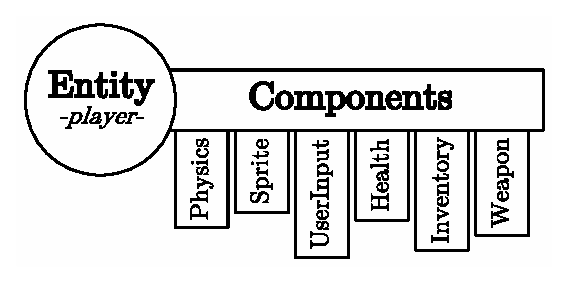
\includegraphics[width=0.8\linewidth]{share/player_entity.eps}
            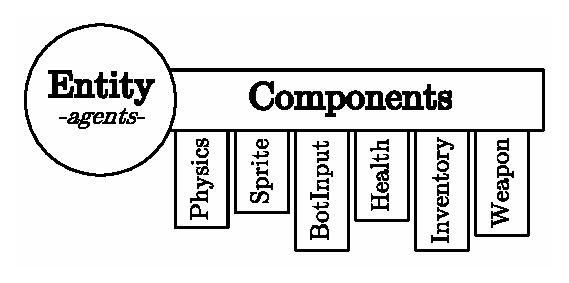
\includegraphics[width=0.8\linewidth]{share/agent_entity.eps}
            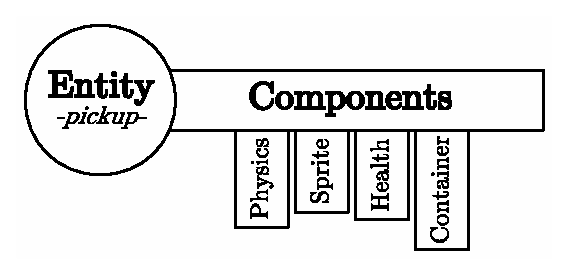
\includegraphics[width=0.8\linewidth]{share/pickup_entity.eps}
            \caption{List of Components in Entity}
            \label{fig:entity_component_system}
        \end{figure}

        Outside the entity, a set of \emph{systems} are running, which manage inter-entity communication such as \emph{path-finding}, \emph{physics}, and \emph{gameplay}. As we touched upon before, these systems are passed as references to the components that are interested in them, allowing for the components to decide what to do with the data provided by the systems without caring about the system's implementation details.

        \begin{figure}[H]
            \centering
            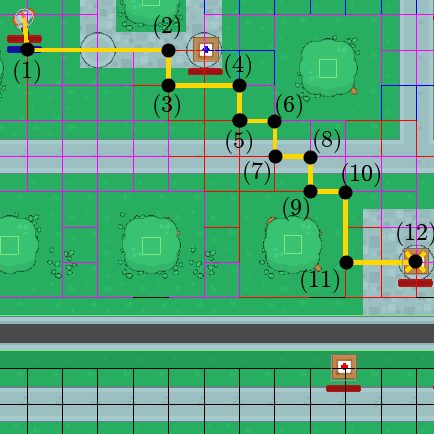
\includegraphics[width=0.7\linewidth]{share/path_finding_stack.png}
            \caption{Visualization of the path finding stack \(\mathcal{S}\). If there are no obstacles in the way (light-of-sight check), the agent takes a straight-line path instead.}
            \label{fig:path_finding_stack}
        \end{figure}

        \twocolumn[{
        \begin{figure}[H]
            \centering
            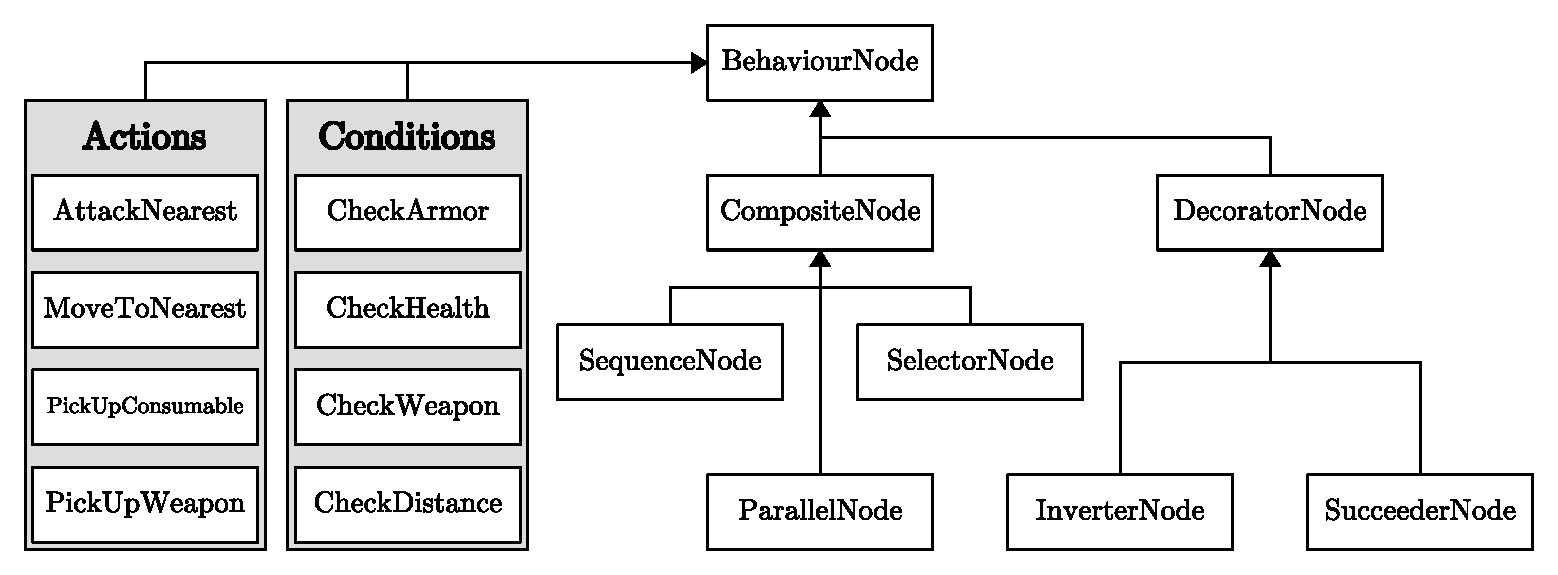
\includegraphics[width=\textwidth]{share/behaviour_tree_uml.eps}
            \label{fig:behaviour_tree_hierarchy}
        \end{figure}
        }]

        \subsection{Behaviour Trees} \label{sec:behaviour_trees_implementation}

        Inside of \texttt{se.sciion.quake2d.ai.behaviour} you'll find the implementation of our BTs. They are specified using inheritance, as in the figure above. In our variant, only the leaves above are non-abstract.

        All are derived from the \texttt{BehaviourNode}, which provides the \emph{State}, and methods for updating states, by evaluating it and its children (if it has any). This is done with the \texttt{tick} function, which is called for each agent's behaviour tree and once for each frame.

        \begin{algorithm}[H]
            \caption{Pseudo-Code for the BT's Tick Step}
            \label{alg:behaviour_tree_update}
            \begin{algorithmic}
                \REQUIRE{some initial \(State\) to the behaviour tree}
                \IF{\(State \neq Running\)}
                    \STATE \(doBehaviourEnter()\)
                \ENDIF
                \STATE \(State \leftarrow doBehaviourUpdate()\)
                \IF{\(State \neq Running\)}
                    \STATE \(doBehaviourExit()\)
                \ENDIF
            \end{algorithmic}
        \end{algorithm}

        Each of these entities' behaviour tree are built from the bottom-up and linked. There is only one \texttt{root} node which needs to be evaluated, since it will recursively evaluate all it's children when requested.

        The standard non-leaf nodes are implemented in a straight-forward way following \cref{sec:behaviour_trees}. Instead, we continue by explaining the \emph{actions} \& \emph{conditions} we have implemented, and how these communicate with the other systems to be able to query the world.

        We've adopted a fairly simple solution, where the leaf-node is given a reference to systems that it wants to communicate with, and the entity owner.

        For example, if a BT wants a \emph{AttackNearest} node beneath a \emph{Succeeder}, we'd first have to hand over a reference to the \emph{path finder} and a \emph{target tag} to the node's constructor, such as: \emph{AttackNearest(path-finder, tag)}. Only after that are we allowed to execute: \emph{SucceederNode(attack-nearest)}, which we can utilize to construct the next parent layer above it.

        Below is a list of all actions and conditions we've implemented in our game, along with a description:

        \begin{itemize}
            \item{\textbf{AttackNearest(\emph{tag}):} finds the closest entity with \emph{tag} and \emph{path find} to it. Shoot with weapon. \emph{Success} if we were able to fire, \emph{false} otherwise.}
            \item{\textbf{MoveToNearest(\emph{tag}):} finds the close entity with \emph{tag} and \emph{path find} to it. Stops when close. \emph{Success} when we're close, \emph{fails} if no valid path.}
            \item{\textbf{PickUpConsumable(\emph{type}):} finds the closest consumable of \emph{type} (\emph{health}, \emph{armor} and \emph{boost}), \emph{path find} to it and \emph{pick it up}. \emph{Fails} if it couldn't.}
            \item{\textbf{PickUpWeapon(\emph{type}):} finds a close weapon of \emph{type} (\emph{shotgun}, \emph{rifle} \& \emph{sniper}). \emph{Path find} to it \& try to \emph{pick it up}. \emph{Succeeds} when picked up.}
        \end{itemize}
        \begin{itemize}
            \item{\textbf{CheckStatus(\emph{ratio, type}):} checks the entity owner's \emph{status} (\emph{health} or \emph{armor}), and returns \emph{Success} if above the \emph{ratio}, or \emph{fail} if its below.}
            \item{\textbf{CheckWeapon(\emph{type}):} checks entity owner's \emph{inventory} for weapon \emph{type}. \emph{Success} if we got it.}
            \item{\textbf{CheckDistance(\emph{tag, r})} checks if entity with \emph{tag} is above \emph{r} units away. \emph{Succeeds} query if so.}
        \end{itemize}

        \clearpage

        \subsection{Genetic Programming} \label{sec:genetic_programming_implementation}

        Since the \textit{genetic programming} has to be done on the trees during runtime we need a way to dynamically generate trees with varying structure and behaviour types. The solution used in this project it by creating a set of \textit{prototype behaviour nodes} \(\mathcal{S}\), one for each node type. This set can then be used to create the trees by building them from the root. The prototypes are implemented using the \textit{prototype design pattern} as presented by \textit{R. Nystrom}~\cite{nystrom2014game}.

        \subsubsection*{Tree generation}

        Each tree is generated by first picking a random node \(n \in \mathcal{S}\) as the tree root and if the node is a \textit{composite}, continue recursively until a complete tree is formed.

        All nodes have an \textit{randomization} function which given on the type of node, randomizes it in different ways. Leaf nodes have an trivial \textit{randomization} function which only tweak parameters such as thresholds and game tags.
        \begin{equation}
        \label{eq:leaf-randomization}
            r(n) \rightarrow \hat{n}
        \end{equation}
        Randomization function for a leaf node.


        Composite nodes \(\mathcal{C} = \{n_0,...,n_i\}\) are randomized recursively, first randomizing the set of children \(\mathcal{C}_r = \{n_0,...,n_m\}, n \in \mathcal{C}\) and \(\mathcal{C}_a = \{n_0,...n_j\}, n \in \mathcal{S}\). \(\mathcal{C}\) is then redefined as \(\mathcal{C} = (\mathcal{C} \cup \mathcal{C}_a)/ \mathcal{C}_r \), adding the set \(\mathcal{C}_a\) and removing the nodes in the set \(\mathcal{C}_r\). Once this is done each child nodes' respective \textit{randomize} function is called 
        \begin{equation}
        \label{eq:composite-randomlization}
            r(\mathcal{C}) \rightarrow \forall_{x} r(n),x \in \mathcal{C}
        \end{equation}
         Randomization function for a composite node.

        \subsubsection*{Tree mutation}

        As with \textit{tree randomization}, the mutation of trees are done in a recursive manner where each node mutate it self and in the case of composite nodes also its children. The mutation differs from randomization in that values only slightly changes with a certain probability, whereas the randomization can completely change all nodes in a tree.
       
        \begin{figure}[H]
            \centering
            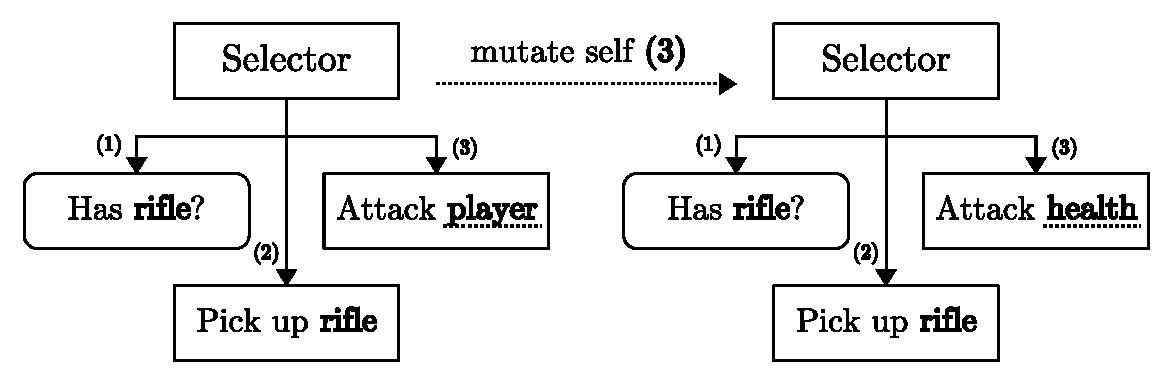
\includegraphics[width=\linewidth]{share/leaf_mutation.eps}
            \caption{Example of Mutation for the Leaf Node}
            \label{fig:leaf_mutation}
        \end{figure}

        \begin{figure}[H]
            \centering
            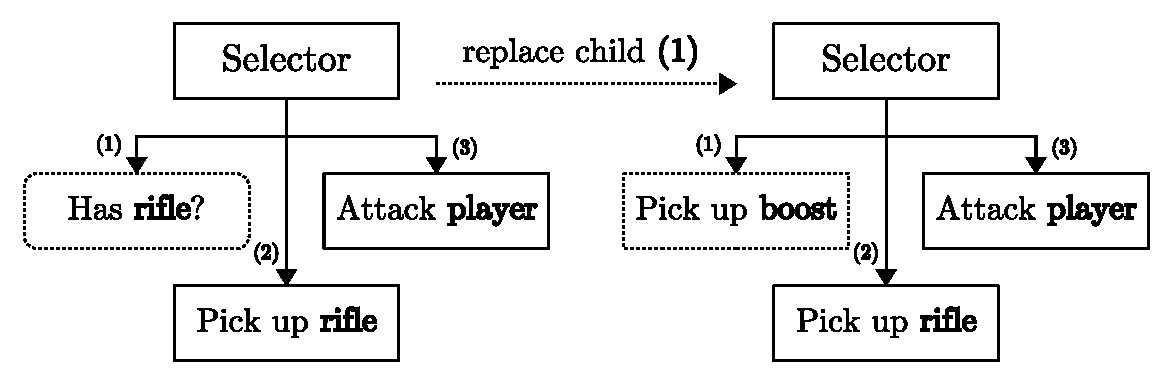
\includegraphics[width=\linewidth]{share/child_replacement.eps}
            \caption{Example of Mutation for Composite Node}
            \label{fig:child_replacement}
        \end{figure}

        As part of the mutation step, trees can also \emph{crossover}. \emph{Crossover} means that two selected sub-trees of two behaviour trees swaps places.
        \begin{figure}[H]
            \centering
            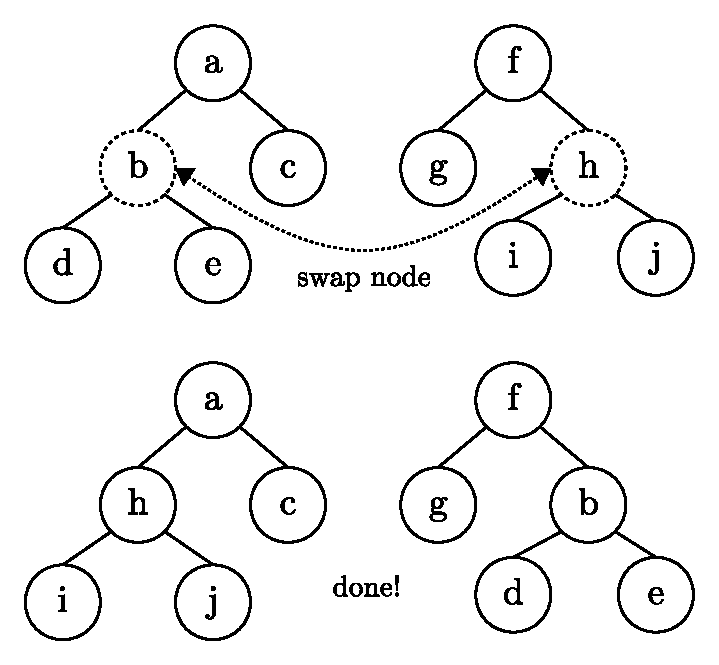
\includegraphics[width=\linewidth]{share/node_swapping.eps}
            \caption{Example of crossover between two trees.}
            \label{fig:child_crossover}
        \end{figure}

        \subsubsection*{Fitness function}
        As alluded to in the theory section, the fitness function is defined as an arbitrary linear combination of game related parameters. The full implementation is described in pseudo-code below.
        \vspace{-0.4em}

        \begin{algorithm}[H]
            \caption{Pseudo-Code for the fitness function}
            \label{alg:fitness_function}
            \begin{algorithmic}
                \REQUIRE {$damage$ being the damage given}
                \REQUIRE {$armor$ begin the armour picked-up}
                \REQUIRE {$weapon$ to be the weapon picked-up}
                \REQUIRE {$kills$ to be the number of agents killed}
                $Score$ = $5 *damage$ + $2 * armor$ + $50 * weapon$ + $1000 * kills$
                \IF {Individual Won}
                    \RETURN $Score + 500$
                \ELSE
                    \RETURN $Score$
                \ENDIF
            \end{algorithmic}
        \end{algorithm}
        \vspace{-0.6em}

        The score is also divided by the number of round each individual played during one generation. This allows for a given individual to test its fitness against multiple adversaries to get a better estimated fitness, a useful detail when fitness evaluation is done against other peers from the same generation.

    \section{Results and Screenshots} \label{sec:results_and_screenshots}

        Below are a couple of in-game screenshots from \emph{Quake 2D}, our testbed for \emph{behaviour tree evolution}. Here we've chosen to show two bots playing against each other in the arena, each of them loaded with a basic hand-made behaviour tree shown in \cref{fig:hand_crafted_behaviour_tree}.

        As can be seen in \cref{fig:behaviour_tree_screenshot}, the environment is composed of \emph{static collidable walls}, \emph{dynamic pick up crates}, \emph{user/agent controlled players}, and \emph{graphical scenery details} based on \emph{tiled textures}. Maps are specified using the \emph{Tiled} editor, which means we can build new environments to test our solution. We've also created a serializer for our behaviour trees, that enables us to save and load behaviour trees to disk.

        Additionally, we've developed several tools for showing our agent's behaviour in real-time. As can be seen, \cref{fig:path_finding_screenshot}, we're able to \emph{visualize path finding information} for the intelligent agents. Here the \emph{yellow line} is the \emph{target path} specified by the \emph{path finding} system given a \emph{target location} (shown as a \emph{yellow cross}) by the \emph{behaviour tree}. In this example, the target is the \emph{rifle pickup crate}. You'll also see a coloured grid being displayed. This tells us something about the state of the \emph{influence map}, where the \emph{blue and red lines} are grids that each agent is able to shoot towards, while \emph{magenta lines} are locations where both agents are able to shoot towards.

        \begin{figure}[H]
            \centering
            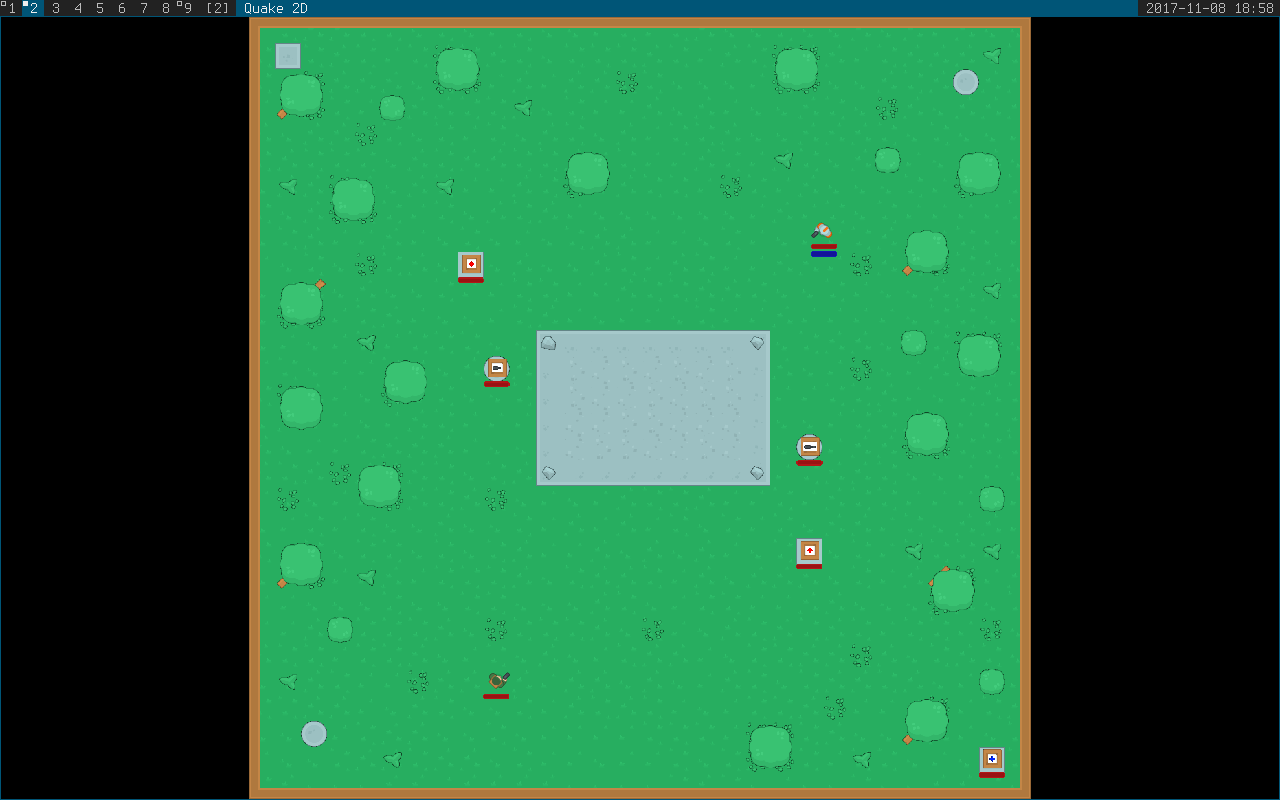
\includegraphics[width=\linewidth]{share/screenshot.png}
            \caption{Screenshot of a Bot vs Bot in Quake 2-D}
            \label{fig:behaviour_tree_screenshot}
        \end{figure}

        For debugging and analyzing agent behaviour, we've also implemented a way to visualize BTs, the one in \cref{fig:hand_crafted_behaviour_tree} from the \cref{fig:path_finding_screenshot} situation, in real-time by using a \emph{Graphviz}\footnote{\url{https://github.com/nidi3/graphviz-java}} library. It opens in a separate window and runs in another thread, where we can see instant changes in the BT's nodes' state.

        \begin{figure}[H]
            \centering
            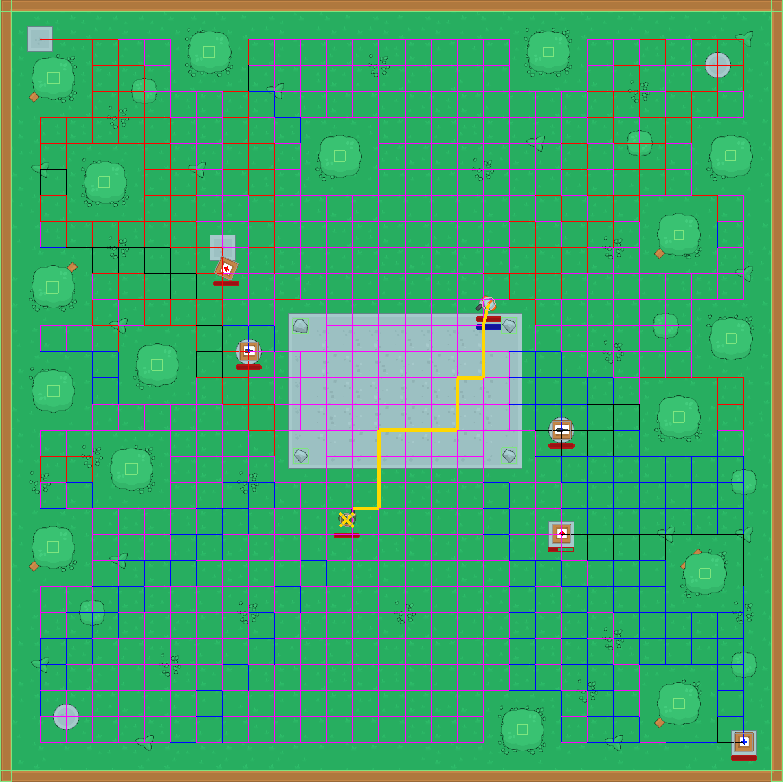
\includegraphics[width=\linewidth]{share/path_finding_screenshot.png}
            \caption{Screenshot of Path Finding in Quake 2-D}
            \label{fig:path_finding_screenshot}
        \end{figure}

        \begin{figure}[H]
            \centering
            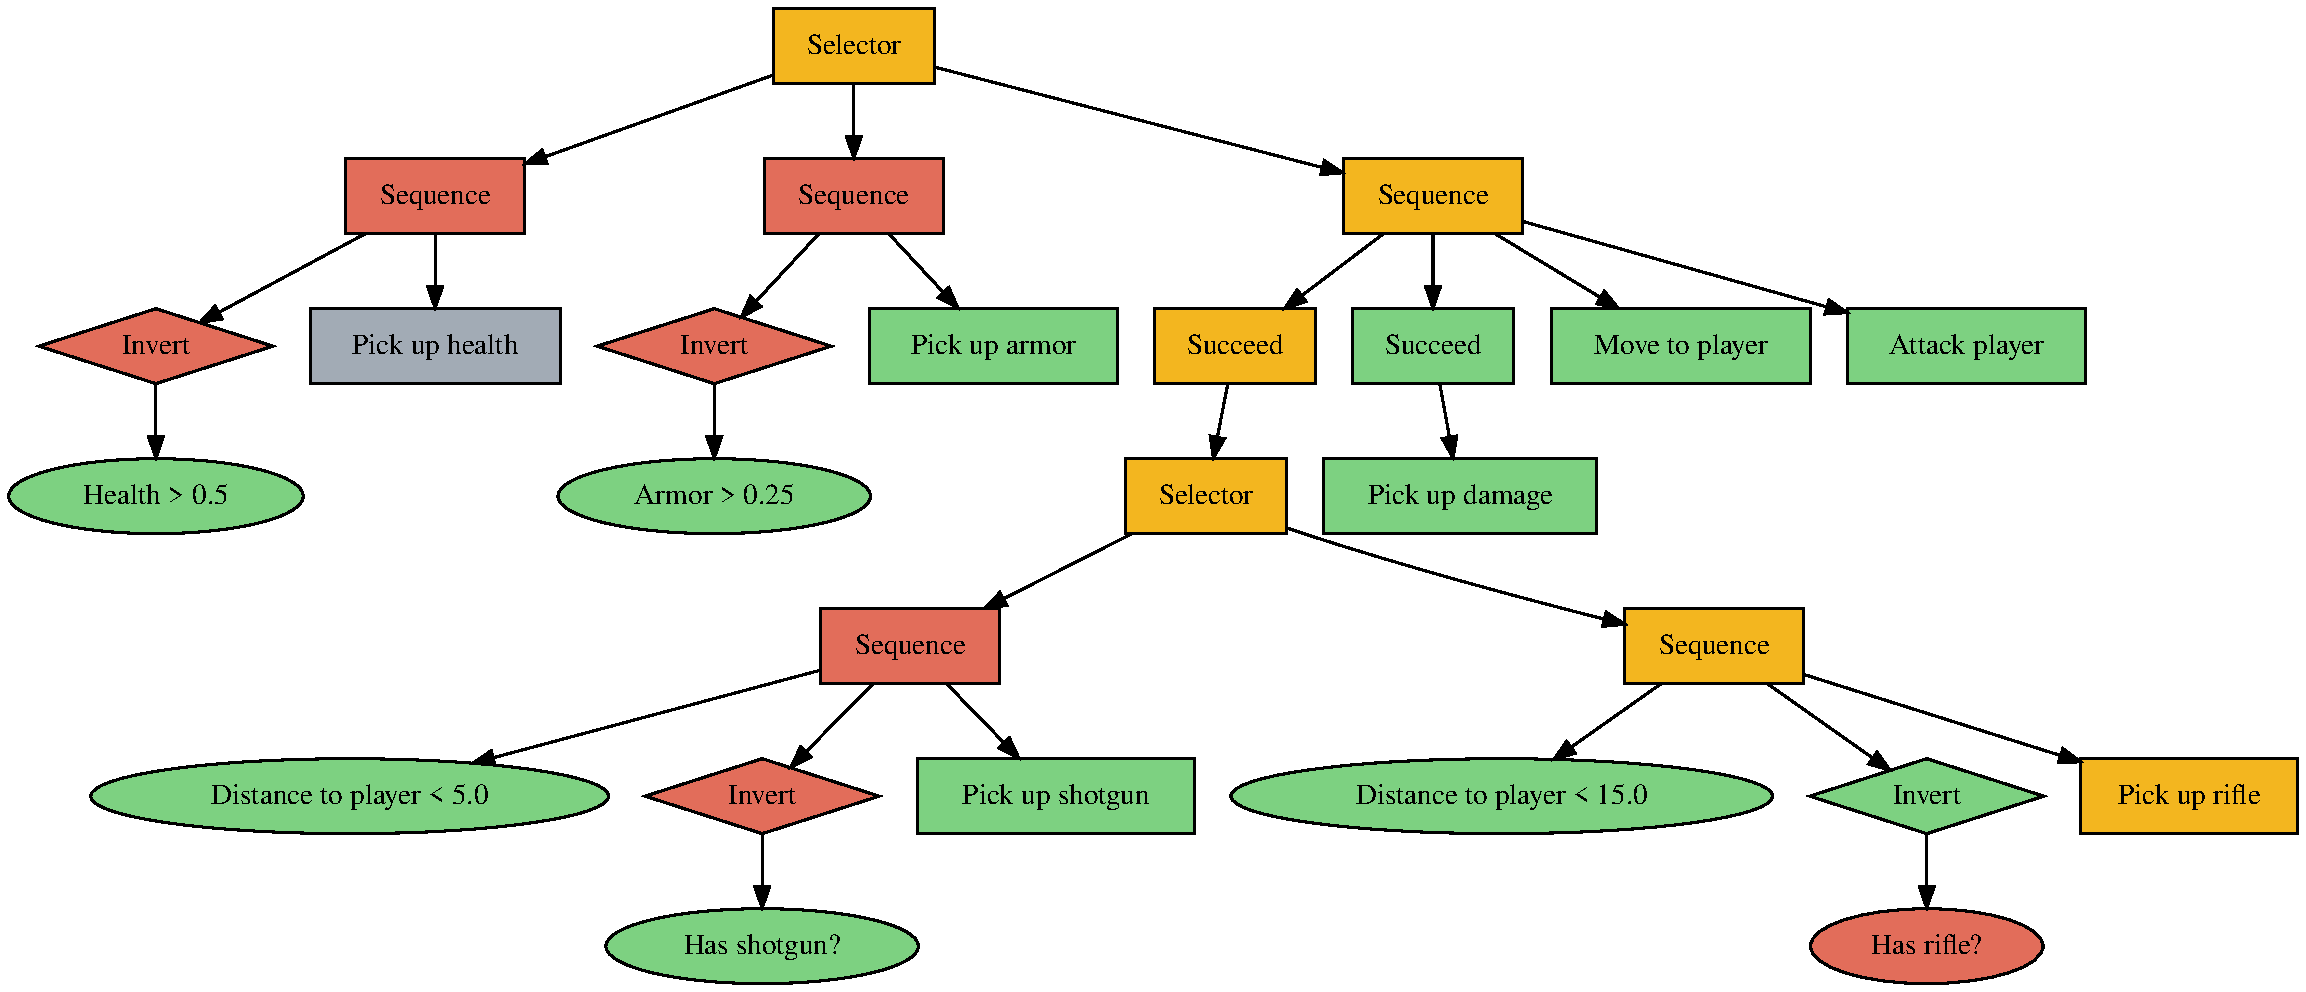
\includegraphics[width=\linewidth]{share/hand_crafted_behaviour_tree.pdf}
            \caption{Hand-Crafted BT (Larger in Appendix)}
            \label{fig:hand_crafted_behaviour_tree}
        \end{figure}

        We've uploaded a video\footnote{\url{https://vimeo.com/Quake2D}} of our solution in action.

        Finally, we present the results from our solution. After generating fifty random individuals for \(\mathcal{P}_0\), we applied genetic programming until we had \(\mathcal{P}_{50}\), the resulting pool of \emph{evolved behaviour trees}. The fitness for each individual in each generation was found by having a match against our crafted behaviour tree, and recording match statistics, used to calculate \(f_i\).

        \subsection{Generated Behaviours} \label{sec:generated_behaviours}

        Each fitness evaluation was performed on a randomly selected hand-crafted level to prevent the behaviour trees getting overfitting to a specific level. 

        \begin{figure}[H]
            \centering
            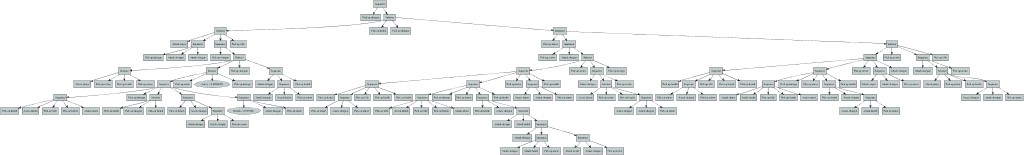
\includegraphics[width=\linewidth]{share/tree-fitness-4750.png}
            \caption{Generated tree with very high fitness (4750)}
            \label{fig:tree_fitness_4075}
        \end{figure}
        As can be seen in the image above. The tree is way to big to provide any significant insight unless interactively evaluated during run time. The fitness score is very close to the limit for the levels used during the fitness evaluation.

        \begin{figure}[H]
            \centering
            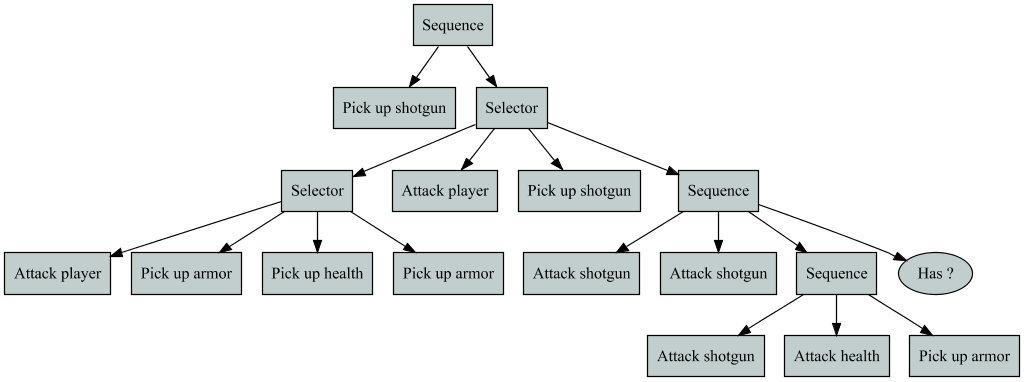
\includegraphics[width=\linewidth]{share/tree-fitness-3780.png}
            \caption{Generated tree with high fitness}
            \label{fig:tree_fitness_3650}
        \end{figure}
        The smaller tree above in fig~\cref{fig:tree_fitness_3650} manages to defeat the hard coded bot on al levels without bloating to unmanageable size. Prior exploration of generated trees indicated that as long as the tree have a \textit{sequence} of \textit{pick-up shotgun} and \textit{attack player}, it would reach an fitness of around \(1000\).

        \twocolumn[{
        \subsection{Behaviour Fitness} \label{sec:behaviour_fitness}

        Looking at the general fitness over generations we can observe how once the behaviour trees routinely defeats its adversary, the mean fitness plateaus and the variance fills the entire range of possible fitness values. When evaluating each tree against random peers, we see something similar but it converges with a slower rate. 

        \begin{figure}[H]
            \centering
            \begin{minipage}{\textwidth}  
                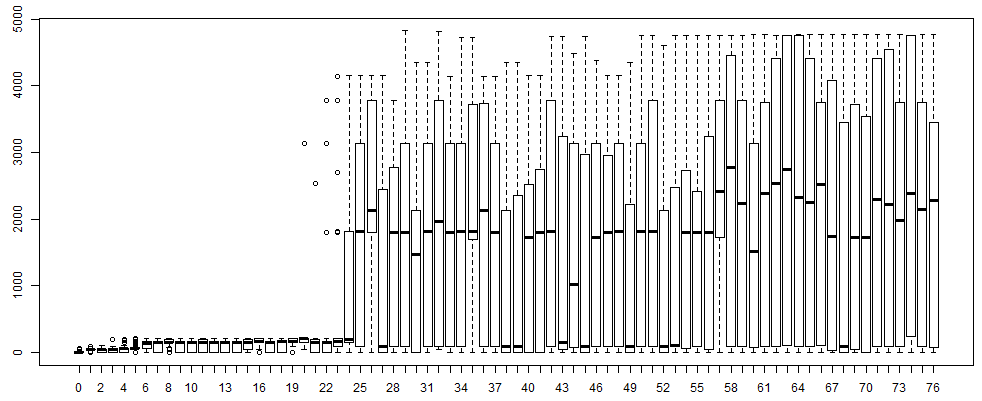
\includegraphics[width=\textwidth]{share/result-againts-bot.png}
                \caption{Fitness over generations when evaluating against a hard-coded bot. Higher score faster is better.}
                \label{fig:fitness-against-bot}
            \end{minipage}
            \begin{minipage}{\textwidth}  
                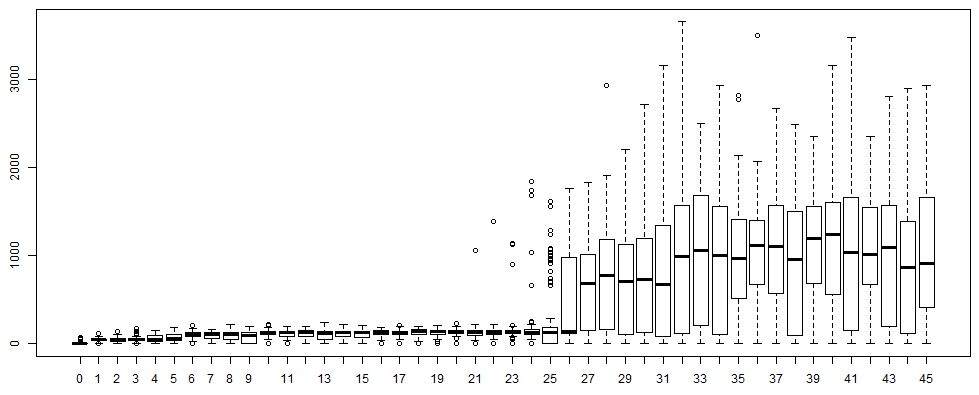
\includegraphics[width=\textwidth]{share/result-random.png}
                \caption{Fitness over generations when evaluating against 2 random peers. Higher score faster is better.}
                \label{fig:fitness-against-random}
            \end{minipage}
        \end{figure}

}]

    \twocolumn[{
        \subsection{Survival Ratio} \label{sec:survival_ratio}
        In the ideal case, the survival rate follows as an consequence of the fitness score. In the two figures above we can see the same trend as in the fitness, the higher the fitness, the higher the survival rate. If this wasn't the case, our fitness evaluation wouldn't provide a good metric for evaluating combat performance.  

        \begin{figure}[H]
            \centering
            \begin{minipage}{\textwidth}  
                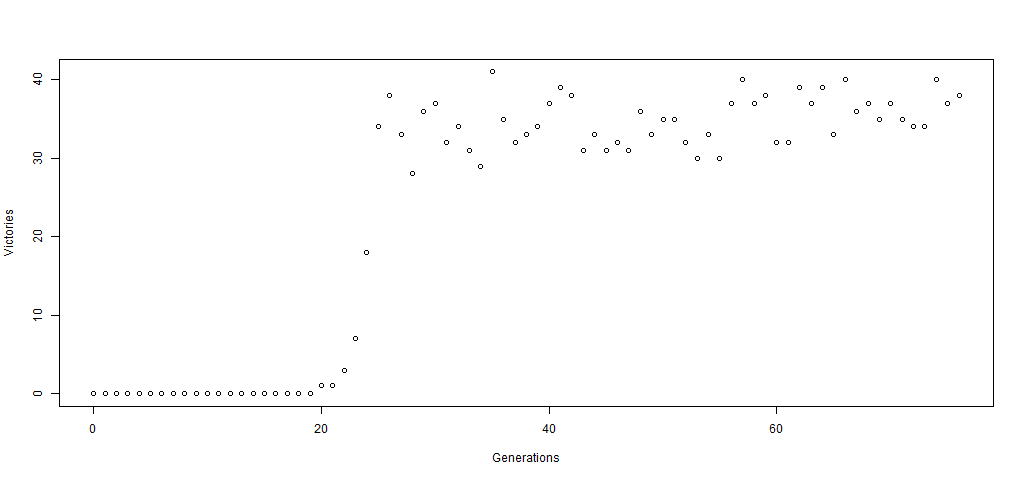
\includegraphics[width=\textwidth]{share/result-victories-against-bot.png}
                \caption{Number of victories for each generation when evaluating against a hard-coded bot. Higher value is better.}
                \label{fig:victory-against-bot}
            \end{minipage}
            \begin{minipage}{\textwidth}  
                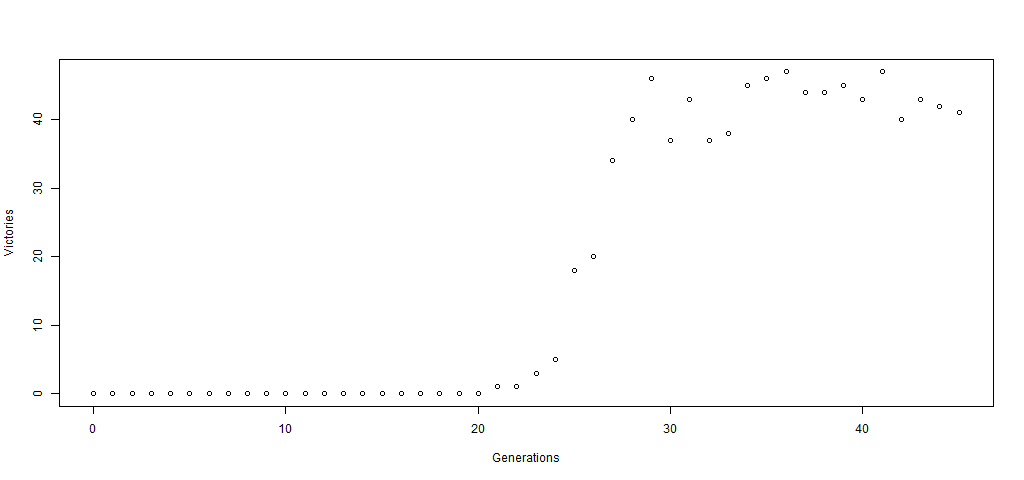
\includegraphics[width=\textwidth]{share/result-victories-random.png}
                \caption{Number of victories for each generations when evaluating against 2 random peers. Higher value is better.}
                \label{fig:victory-against-random}
            \end{minipage}
        \end{figure}

        }]

        \clearpage

    \section{Discussion and Outlook} \label{sec:discussion_and_outlook}

    There are some main areas of the project which merits further analysis, we start with the results section and what can be extrapolated from the fitness and survival score. Afterwards we look at some limitations of project, related work, and end with future improvements.

    \subsection*{Convergence Rate}

    As can be seen in the plots in the result section, the evolutionary algorithm converges to an high game proficiency in just a couple of generations. The fact that it manges to this can reflect poorly on our skills as game designers. Since we can expect that the more complex behaviours required to proficiently play a game, the more generations it will take until it produces such behaviour trees. It can also be viewed as the fitness function, tree mutation, and pool of possible actions being well tuned to the specific requirements of this project. Which one is the correct interpretation is left to the reader. 

    A possible explanation to the different convergence rates when evaluating against a hard-coded tree or adversarial peers is the stochastic nature of both level selection and the randomized adversary. The adversarial peer should be much closer in performance compared to the hard-coded tree. Once trees which can defeat the hard-coded bot have been generated, additional fitness can only be reached by overfitting to the given level selection. The trees with peer evaluation on the other hand can't find a solution on how to reliably defeat the enemy. The adversary co-evolves with them which makes it very hard to find a ``holy-bullet'' since the generation after everyone has it.

    \subsection*{Limitations}

    When tested against a human player the generated behaviours becomes very hard to defeat. Since we decided on very high level actions, the produced behaviours often appears clunky compared to a human player. For example, two bots might decide to walk to the same \emph{health} pick-up when both have a very low \emph{health} instead of just killing each other. 


    \subsection*{Related Work}

    The genetic programming solution was initially based on the work by~\cite{colledanchise2015learning}. The solution proposed in the paper did not pan out in our case since they use an selection heuristic during the mutation phase, allowing for higher fitness increase over fewer generations. The paper also used primitive actions which would not scale to the type of game used in this project without \emph{very} large behaviour trees. With this said, it seems like low-level actions might produce more ``clutch'' behaviours in this kind of fast-paced games. 


    \subsection*{Future Work}

    Extract the behaviour tree part and genetic programming as an independent library. Use heuristics during the creation of each new generation. Add additional behaviours and game mechanics to the project. Have it compete with it self instead of an hard-coded adversary. Have the fitness evaluation run in headless mode. \footnote{Repository: \url{https://github.com/sci10n/Quake2D}}

    \nocite{*} % Include all.
    \bibliographystyle{abbrv}
    \bibliography{report}

    \onecolumn
    \clearpage

    \appendix

    \thispagestyle{empty}

    \begin{figure}[H]
        \centering
        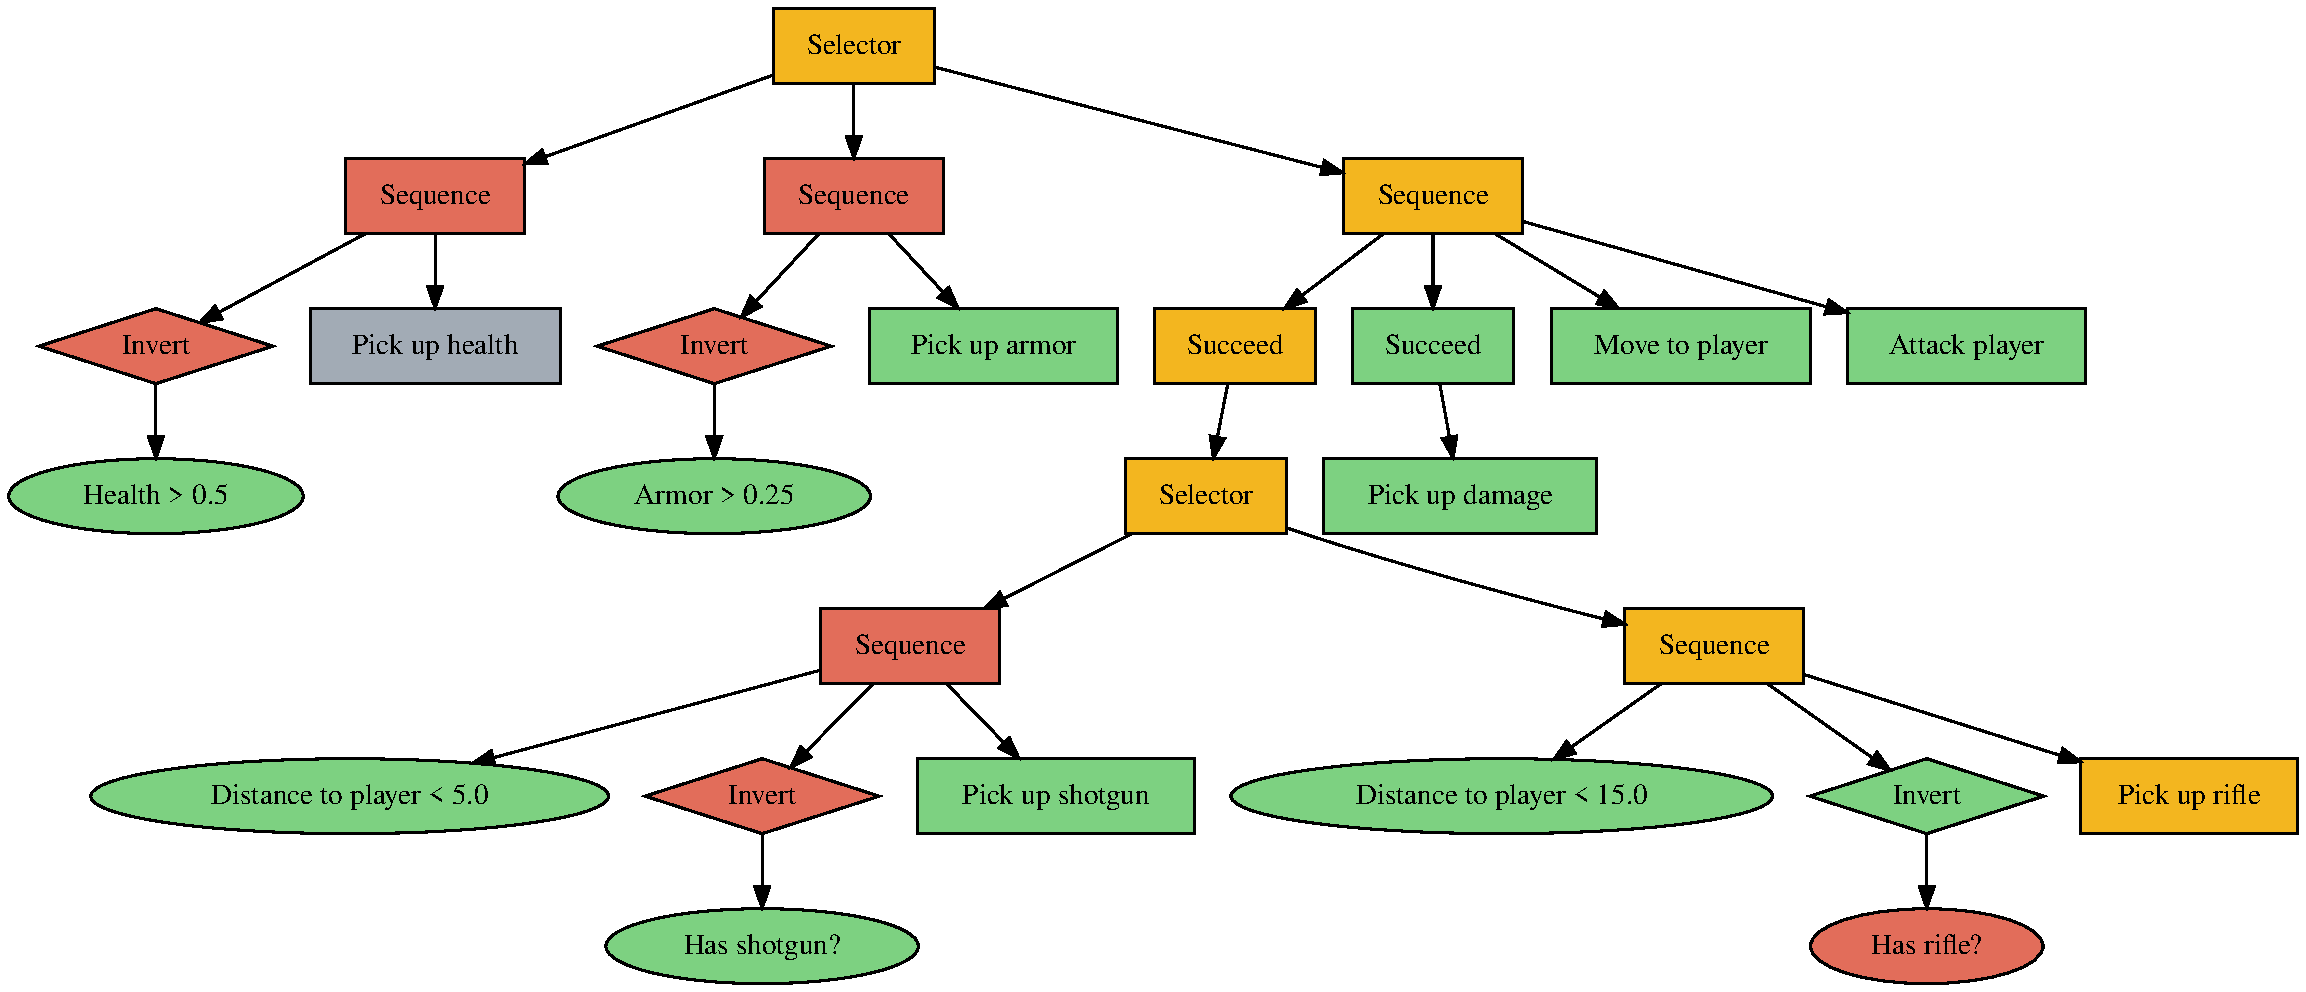
\includegraphics[angle=90,height=0.98\textheight]{share/hand_crafted_behaviour_tree.pdf}
    \end{figure}

    \clearpage

    \thispagestyle{empty}

    \begin{figure}[H]
        \centering
        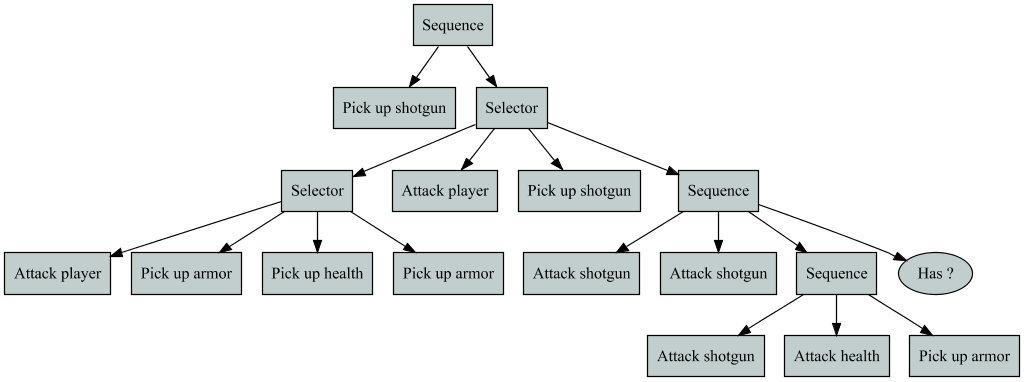
\includegraphics[angle=90,height=0.98\textheight]{share/tree-fitness-3780.png}
    \end{figure}

\end{document}
